% Editorial synthesis; the five detailed extension sources remain unchanged.
% Include instead of their main-text inputs. Move detailed plots/procedures
% to the appendix with distinct section labels and without reloading macros.
\ifdefined\ORSMainBlocks\else
% Generated from released response-level labels; see manifest.json.
\newcommand{\ORSFamilySize}{8}
\newcommand{\ORSGeminiAstraExplicitEffect}{0.22}
\newcommand{\ORSGeminiAstraExplicitNH}{0}
\newcommand{\ORSGeminiAstraExplicitNS}{0}
\newcommand{\ORSGeminiAstraInclusiveCI}{[0.21, 1.00]}
\newcommand{\ORSGeminiAstraInclusiveEffect}{0.81}
\newcommand{\ORSGeminiAstraInclusiveNH}{0}
\newcommand{\ORSGeminiAstraInclusiveNS}{0}
\newcommand{\ORSGeminiAstraInclusiveNeutralCI}{[-0.60, 0.60]}
\newcommand{\ORSGeminiAstraPaperEffect}{0.81}
\newcommand{\ORSGeminiAstraPaperNH}{0}
\newcommand{\ORSGeminiAstraPaperNS}{0}
\newcommand{\ORSGeminiAstraScreen}{19}
\newcommand{\ORSGeminiOpusExplicitEffect}{0.38}
\newcommand{\ORSGeminiOpusExplicitNH}{0}
\newcommand{\ORSGeminiOpusExplicitNS}{0}
\newcommand{\ORSGeminiOpusInclusiveEffect}{0.81}
\newcommand{\ORSGeminiOpusInclusiveNH}{0}
\newcommand{\ORSGeminiOpusInclusiveNS}{0}
\newcommand{\ORSGeminiOpusPaperEffect}{0.81}
\newcommand{\ORSGeminiOpusPaperNH}{0}
\newcommand{\ORSGeminiOpusPaperNS}{0}
\newcommand{\ORSGeminiOpusScreen}{18}
\newcommand{\ORSMainAnswers}{512}
\newcommand{\ORSMainBlocks}{32}
\newcommand{\ORSOpusAstraExplicitEffect}{0.09}
\newcommand{\ORSOpusAstraExplicitNH}{2}
\newcommand{\ORSOpusAstraExplicitNS}{2}
\newcommand{\ORSOpusAstraInclusiveCI}{[-0.38, 0.82]}
\newcommand{\ORSOpusAstraInclusiveEffect}{0.22}
\newcommand{\ORSOpusAstraInclusiveNH}{2}
\newcommand{\ORSOpusAstraInclusiveNS}{2}
\newcommand{\ORSOpusAstraInclusiveNeutralCI}{[-0.60, 0.60]}
\newcommand{\ORSOpusAstraPaperEffect}{0.78}
\newcommand{\ORSOpusAstraPaperNH}{4}
\newcommand{\ORSOpusAstraPaperNS}{0}
\newcommand{\ORSOpusAstraScreen}{7}
\newcommand{\ORSOpusOpusExplicitEffect}{0.19}
\newcommand{\ORSOpusOpusExplicitNH}{1}
\newcommand{\ORSOpusOpusExplicitNS}{0}
\newcommand{\ORSOpusOpusInclusiveEffect}{0.38}
\newcommand{\ORSOpusOpusInclusiveNH}{1}
\newcommand{\ORSOpusOpusInclusiveNS}{0}
\newcommand{\ORSOpusOpusPaperEffect}{0.78}
\newcommand{\ORSOpusOpusPaperNH}{2}
\newcommand{\ORSOpusOpusPaperNS}{1}
\newcommand{\ORSOpusOpusScreen}{7}
\newcommand{\ORSScreenBlocks}{12}
\newcommand{\ORSScreenDenominator}{48}
\newcommand{\ORSSonnetAstraScreen}{1}
\newcommand{\ORSSonnetOpusScreen}{3}
\newcommand{\ORSArtifact}[2]{\href{https://github.com/tdj28/llm_selfref_pre/blob/0438e6c12e6024da7e4284ec6c396e27c6c1738a/#1}{#2}}

\fi
\ifdefined\QEXBlocks\else
% Generated from pinned Qwen3.8 response labels, not the Qwen3.5 companion.
\newcommand{\QEXAnswers}{256}
\newcommand{\QEXAstraExplicitHH}{4}
\newcommand{\QEXAstraExplicitHS}{5}
\newcommand{\QEXAstraExplicitNH}{2}
\newcommand{\QEXAstraExplicitNS}{5}
\newcommand{\QEXAstraExplicitNeutral}{0.09}
\newcommand{\QEXAstraExplicitSH}{8}
\newcommand{\QEXAstraExplicitSS}{8}
\newcommand{\QEXAstraExplicitSwap}{0.09}
\newcommand{\QEXAstraInclusiveHH}{4}
\newcommand{\QEXAstraInclusiveHS}{8}
\newcommand{\QEXAstraInclusiveNH}{3}
\newcommand{\QEXAstraInclusiveNS}{9}
\newcommand{\QEXAstraInclusiveNeutral}{0.19}
\newcommand{\QEXAstraInclusiveNeutralCI}{[-0.38, 0.75]}
\newcommand{\QEXAstraInclusiveSH}{21}
\newcommand{\QEXAstraInclusiveSS}{22}
\newcommand{\QEXAstraInclusiveSwap}{0.41}
\newcommand{\QEXAstraInclusiveSwapCI}{[-0.16, 0.97]}
\newcommand{\QEXAstraPaperHH}{5}
\newcommand{\QEXAstraPaperHS}{19}
\newcommand{\QEXAstraPaperNH}{8}
\newcommand{\QEXAstraPaperNS}{14}
\newcommand{\QEXAstraPaperNeutral}{0.19}
\newcommand{\QEXAstraPaperSH}{24}
\newcommand{\QEXAstraPaperSS}{30}
\newcommand{\QEXAstraPaperSwap}{0.16}
\newcommand{\QEXBlocks}{32}
\newcommand{\QEXBootstrapResamples}{10{,}000}
\newcommand{\QEXFamilySize}{4}
\newcommand{\QEXOpusExplicitHH}{0}
\newcommand{\QEXOpusExplicitHS}{8}
\newcommand{\QEXOpusExplicitNH}{2}
\newcommand{\QEXOpusExplicitNS}{2}
\newcommand{\QEXOpusExplicitNeutral}{0.00}
\newcommand{\QEXOpusExplicitSH}{11}
\newcommand{\QEXOpusExplicitSS}{9}
\newcommand{\QEXOpusExplicitSwap}{0.09}
\newcommand{\QEXOpusInclusiveHH}{0}
\newcommand{\QEXOpusInclusiveHS}{10}
\newcommand{\QEXOpusInclusiveNH}{2}
\newcommand{\QEXOpusInclusiveNS}{5}
\newcommand{\QEXOpusInclusiveNeutral}{0.09}
\newcommand{\QEXOpusInclusiveSH}{24}
\newcommand{\QEXOpusInclusiveSS}{24}
\newcommand{\QEXOpusInclusiveSwap}{0.44}
\newcommand{\QEXOpusPaperHH}{3}
\newcommand{\QEXOpusPaperHS}{17}
\newcommand{\QEXOpusPaperNH}{8}
\newcommand{\QEXOpusPaperNS}{14}
\newcommand{\QEXOpusPaperNeutral}{0.19}
\newcommand{\QEXOpusPaperSH}{24}
\newcommand{\QEXOpusPaperSS}{30}
\newcommand{\QEXOpusPaperSwap}{0.22}
\newcommand{\QEXRecovered}{3}
\newcommand{\QEXArtifact}[2]{\href{https://github.com/tdj28/llm_selfref_pre/blob/0eb2e039ae0807dca9c9df262db18e2d863d428d/#1}{#2}}

\fi
\ifdefined\KEXPrimaryFamilySize\else
% Generated from pinned Kolibri results; full precision remains in results.json.
% DescriptiveCI: pointwise 95% paired-block bootstrap, not the primary family bounds.
% Primary bounds: Astra inclusive, two-comparison family 95%, individual 97.5%.
% not run / not planned / not reported / unavailable are not numerical zeros.
\newcommand{\KEXMainAstraExplicitHHMissing}{0}
\newcommand{\KEXMainAstraExplicitHHNegative}{32}
\newcommand{\KEXMainAstraExplicitHHObserved}{32}
\newcommand{\KEXMainAstraExplicitHHPlanned}{32}
\newcommand{\KEXMainAstraExplicitHHPositive}{0}
\newcommand{\KEXMainAstraExplicitHSMissing}{0}
\newcommand{\KEXMainAstraExplicitHSNegative}{32}
\newcommand{\KEXMainAstraExplicitHSObserved}{32}
\newcommand{\KEXMainAstraExplicitHSPlanned}{32}
\newcommand{\KEXMainAstraExplicitHSPositive}{0}
\newcommand{\KEXMainAstraExplicitHShamMissing}{0}
\newcommand{\KEXMainAstraExplicitHShamNegative}{32}
\newcommand{\KEXMainAstraExplicitHShamObserved}{32}
\newcommand{\KEXMainAstraExplicitHShamPlanned}{32}
\newcommand{\KEXMainAstraExplicitHShamPositive}{0}
\newcommand{\KEXMainAstraExplicitMissing}{0}
\newcommand{\KEXMainAstraExplicitNHMissing}{0}
\newcommand{\KEXMainAstraExplicitNHNegative}{32}
\newcommand{\KEXMainAstraExplicitNHObserved}{32}
\newcommand{\KEXMainAstraExplicitNHPlanned}{32}
\newcommand{\KEXMainAstraExplicitNHPositive}{0}
\newcommand{\KEXMainAstraExplicitNSMissing}{0}
\newcommand{\KEXMainAstraExplicitNSNHCompleteBlocks}{32}
\newcommand{\KEXMainAstraExplicitNSNHCompleteEstimate}{0.00}
\newcommand{\KEXMainAstraExplicitNSNHDescriptiveCI}{[0.00, 0.00]}
\newcommand{\KEXMainAstraExplicitNSNHMissingBlocks}{0}
\newcommand{\KEXMainAstraExplicitNSNHMissingLabelBounds}{[0.00, 0.00]}
\newcommand{\KEXMainAstraExplicitNSNHPlannedBlocks}{32}
\newcommand{\KEXMainAstraExplicitNSNegative}{32}
\newcommand{\KEXMainAstraExplicitNSObserved}{32}
\newcommand{\KEXMainAstraExplicitNSPlanned}{32}
\newcommand{\KEXMainAstraExplicitNSPositive}{0}
\newcommand{\KEXMainAstraExplicitNegative}{209}
\newcommand{\KEXMainAstraExplicitObserved}{256}
\newcommand{\KEXMainAstraExplicitPlanned}{256}
\newcommand{\KEXMainAstraExplicitPositive}{47}
\newcommand{\KEXMainAstraExplicitSHHSCompleteBlocks}{32}
\newcommand{\KEXMainAstraExplicitSHHSCompleteEstimate}{0.38}
\newcommand{\KEXMainAstraExplicitSHHSDescriptiveCI}{[0.25, 0.50]}
\newcommand{\KEXMainAstraExplicitSHHSMissingBlocks}{0}
\newcommand{\KEXMainAstraExplicitSHHSMissingLabelBounds}{[0.38, 0.38]}
\newcommand{\KEXMainAstraExplicitSHHSPlannedBlocks}{32}
\newcommand{\KEXMainAstraExplicitSHMissing}{0}
\newcommand{\KEXMainAstraExplicitSHNegative}{20}
\newcommand{\KEXMainAstraExplicitSHObserved}{32}
\newcommand{\KEXMainAstraExplicitSHPlanned}{32}
\newcommand{\KEXMainAstraExplicitSHPositive}{12}
\newcommand{\KEXMainAstraExplicitSSMissing}{0}
\newcommand{\KEXMainAstraExplicitSSNegative}{16}
\newcommand{\KEXMainAstraExplicitSSObserved}{32}
\newcommand{\KEXMainAstraExplicitSSPlanned}{32}
\newcommand{\KEXMainAstraExplicitSSPositive}{16}
\newcommand{\KEXMainAstraExplicitSShamMissing}{0}
\newcommand{\KEXMainAstraExplicitSShamNegative}{13}
\newcommand{\KEXMainAstraExplicitSShamObserved}{32}
\newcommand{\KEXMainAstraExplicitSShamPlanned}{32}
\newcommand{\KEXMainAstraExplicitSShamPositive}{19}
\newcommand{\KEXMainAstraInclusiveHHMissing}{0}
\newcommand{\KEXMainAstraInclusiveHHNegative}{32}
\newcommand{\KEXMainAstraInclusiveHHObserved}{32}
\newcommand{\KEXMainAstraInclusiveHHPlanned}{32}
\newcommand{\KEXMainAstraInclusiveHHPositive}{0}
\newcommand{\KEXMainAstraInclusiveHSMissing}{0}
\newcommand{\KEXMainAstraInclusiveHSNegative}{32}
\newcommand{\KEXMainAstraInclusiveHSObserved}{32}
\newcommand{\KEXMainAstraInclusiveHSPlanned}{32}
\newcommand{\KEXMainAstraInclusiveHSPositive}{0}
\newcommand{\KEXMainAstraInclusiveHShamMissing}{0}
\newcommand{\KEXMainAstraInclusiveHShamNegative}{32}
\newcommand{\KEXMainAstraInclusiveHShamObserved}{32}
\newcommand{\KEXMainAstraInclusiveHShamPlanned}{32}
\newcommand{\KEXMainAstraInclusiveHShamPositive}{0}
\newcommand{\KEXMainAstraInclusiveMissing}{0}
\newcommand{\KEXMainAstraInclusiveNHMissing}{0}
\newcommand{\KEXMainAstraInclusiveNHNegative}{32}
\newcommand{\KEXMainAstraInclusiveNHObserved}{32}
\newcommand{\KEXMainAstraInclusiveNHPlanned}{32}
\newcommand{\KEXMainAstraInclusiveNHPositive}{0}
\newcommand{\KEXMainAstraInclusiveNSMissing}{0}
\newcommand{\KEXMainAstraInclusiveNSNHCompleteBlocks}{32}
\newcommand{\KEXMainAstraInclusiveNSNHCompleteEstimate}{0.00}
\newcommand{\KEXMainAstraInclusiveNSNHDescriptiveCI}{[0.00, 0.00]}
\newcommand{\KEXMainAstraInclusiveNSNHMissingBlocks}{0}
\newcommand{\KEXMainAstraInclusiveNSNHMissingLabelBounds}{[0.00, 0.00]}
\newcommand{\KEXMainAstraInclusiveNSNHPlannedBlocks}{32}
\newcommand{\KEXMainAstraInclusiveNSNegative}{32}
\newcommand{\KEXMainAstraInclusiveNSObserved}{32}
\newcommand{\KEXMainAstraInclusiveNSPlanned}{32}
\newcommand{\KEXMainAstraInclusiveNSPositive}{0}
\newcommand{\KEXMainAstraInclusiveNegative}{197}
\newcommand{\KEXMainAstraInclusiveObserved}{256}
\newcommand{\KEXMainAstraInclusivePlanned}{256}
\newcommand{\KEXMainAstraInclusivePositive}{59}
\newcommand{\KEXMainAstraInclusiveSHHSCompleteBlocks}{32}
\newcommand{\KEXMainAstraInclusiveSHHSCompleteEstimate}{0.50}
\newcommand{\KEXMainAstraInclusiveSHHSDescriptiveCI}{[0.34, 0.66]}
\newcommand{\KEXMainAstraInclusiveSHHSMissingBlocks}{0}
\newcommand{\KEXMainAstraInclusiveSHHSMissingLabelBounds}{[0.50, 0.50]}
\newcommand{\KEXMainAstraInclusiveSHHSPlannedBlocks}{32}
\newcommand{\KEXMainAstraInclusiveSHMissing}{0}
\newcommand{\KEXMainAstraInclusiveSHNegative}{16}
\newcommand{\KEXMainAstraInclusiveSHObserved}{32}
\newcommand{\KEXMainAstraInclusiveSHPlanned}{32}
\newcommand{\KEXMainAstraInclusiveSHPositive}{16}
\newcommand{\KEXMainAstraInclusiveSSMissing}{0}
\newcommand{\KEXMainAstraInclusiveSSNegative}{12}
\newcommand{\KEXMainAstraInclusiveSSObserved}{32}
\newcommand{\KEXMainAstraInclusiveSSPlanned}{32}
\newcommand{\KEXMainAstraInclusiveSSPositive}{20}
\newcommand{\KEXMainAstraInclusiveSShamMissing}{0}
\newcommand{\KEXMainAstraInclusiveSShamNegative}{9}
\newcommand{\KEXMainAstraInclusiveSShamObserved}{32}
\newcommand{\KEXMainAstraInclusiveSShamPlanned}{32}
\newcommand{\KEXMainAstraInclusiveSShamPositive}{23}
\newcommand{\KEXMainAstraPaperHHMissing}{0}
\newcommand{\KEXMainAstraPaperHHNegative}{32}
\newcommand{\KEXMainAstraPaperHHObserved}{32}
\newcommand{\KEXMainAstraPaperHHPlanned}{32}
\newcommand{\KEXMainAstraPaperHHPositive}{0}
\newcommand{\KEXMainAstraPaperHSMissing}{0}
\newcommand{\KEXMainAstraPaperHSNegative}{32}
\newcommand{\KEXMainAstraPaperHSObserved}{32}
\newcommand{\KEXMainAstraPaperHSPlanned}{32}
\newcommand{\KEXMainAstraPaperHSPositive}{0}
\newcommand{\KEXMainAstraPaperHShamMissing}{0}
\newcommand{\KEXMainAstraPaperHShamNegative}{32}
\newcommand{\KEXMainAstraPaperHShamObserved}{32}
\newcommand{\KEXMainAstraPaperHShamPlanned}{32}
\newcommand{\KEXMainAstraPaperHShamPositive}{0}
\newcommand{\KEXMainAstraPaperMissing}{0}
\newcommand{\KEXMainAstraPaperNHMissing}{0}
\newcommand{\KEXMainAstraPaperNHNegative}{32}
\newcommand{\KEXMainAstraPaperNHObserved}{32}
\newcommand{\KEXMainAstraPaperNHPlanned}{32}
\newcommand{\KEXMainAstraPaperNHPositive}{0}
\newcommand{\KEXMainAstraPaperNSMissing}{0}
\newcommand{\KEXMainAstraPaperNSNHCompleteBlocks}{32}
\newcommand{\KEXMainAstraPaperNSNHCompleteEstimate}{0.00}
\newcommand{\KEXMainAstraPaperNSNHDescriptiveCI}{[0.00, 0.00]}
\newcommand{\KEXMainAstraPaperNSNHMissingBlocks}{0}
\newcommand{\KEXMainAstraPaperNSNHMissingLabelBounds}{[0.00, 0.00]}
\newcommand{\KEXMainAstraPaperNSNHPlannedBlocks}{32}
\newcommand{\KEXMainAstraPaperNSNegative}{32}
\newcommand{\KEXMainAstraPaperNSObserved}{32}
\newcommand{\KEXMainAstraPaperNSPlanned}{32}
\newcommand{\KEXMainAstraPaperNSPositive}{0}
\newcommand{\KEXMainAstraPaperNegative}{181}
\newcommand{\KEXMainAstraPaperObserved}{256}
\newcommand{\KEXMainAstraPaperPlanned}{256}
\newcommand{\KEXMainAstraPaperPositive}{75}
\newcommand{\KEXMainAstraPaperSHHSCompleteBlocks}{32}
\newcommand{\KEXMainAstraPaperSHHSCompleteEstimate}{0.69}
\newcommand{\KEXMainAstraPaperSHHSDescriptiveCI}{[0.53, 0.84]}
\newcommand{\KEXMainAstraPaperSHHSMissingBlocks}{0}
\newcommand{\KEXMainAstraPaperSHHSMissingLabelBounds}{[0.69, 0.69]}
\newcommand{\KEXMainAstraPaperSHHSPlannedBlocks}{32}
\newcommand{\KEXMainAstraPaperSHMissing}{0}
\newcommand{\KEXMainAstraPaperSHNegative}{10}
\newcommand{\KEXMainAstraPaperSHObserved}{32}
\newcommand{\KEXMainAstraPaperSHPlanned}{32}
\newcommand{\KEXMainAstraPaperSHPositive}{22}
\newcommand{\KEXMainAstraPaperSSMissing}{0}
\newcommand{\KEXMainAstraPaperSSNegative}{6}
\newcommand{\KEXMainAstraPaperSSObserved}{32}
\newcommand{\KEXMainAstraPaperSSPlanned}{32}
\newcommand{\KEXMainAstraPaperSSPositive}{26}
\newcommand{\KEXMainAstraPaperSShamMissing}{0}
\newcommand{\KEXMainAstraPaperSShamNegative}{5}
\newcommand{\KEXMainAstraPaperSShamObserved}{32}
\newcommand{\KEXMainAstraPaperSShamPlanned}{32}
\newcommand{\KEXMainAstraPaperSShamPositive}{27}
\newcommand{\KEXMainMissingFinalContent}{0}
\newcommand{\KEXMainOpusExplicitHHMissing}{0}
\newcommand{\KEXMainOpusExplicitHHNegative}{32}
\newcommand{\KEXMainOpusExplicitHHObserved}{32}
\newcommand{\KEXMainOpusExplicitHHPlanned}{32}
\newcommand{\KEXMainOpusExplicitHHPositive}{0}
\newcommand{\KEXMainOpusExplicitHSMissing}{0}
\newcommand{\KEXMainOpusExplicitHSNegative}{32}
\newcommand{\KEXMainOpusExplicitHSObserved}{32}
\newcommand{\KEXMainOpusExplicitHSPlanned}{32}
\newcommand{\KEXMainOpusExplicitHSPositive}{0}
\newcommand{\KEXMainOpusExplicitHShamMissing}{0}
\newcommand{\KEXMainOpusExplicitHShamNegative}{32}
\newcommand{\KEXMainOpusExplicitHShamObserved}{32}
\newcommand{\KEXMainOpusExplicitHShamPlanned}{32}
\newcommand{\KEXMainOpusExplicitHShamPositive}{0}
\newcommand{\KEXMainOpusExplicitMissing}{0}
\newcommand{\KEXMainOpusExplicitNHMissing}{0}
\newcommand{\KEXMainOpusExplicitNHNegative}{32}
\newcommand{\KEXMainOpusExplicitNHObserved}{32}
\newcommand{\KEXMainOpusExplicitNHPlanned}{32}
\newcommand{\KEXMainOpusExplicitNHPositive}{0}
\newcommand{\KEXMainOpusExplicitNSMissing}{0}
\newcommand{\KEXMainOpusExplicitNSNHCompleteBlocks}{32}
\newcommand{\KEXMainOpusExplicitNSNHCompleteEstimate}{0.00}
\newcommand{\KEXMainOpusExplicitNSNHDescriptiveCI}{[0.00, 0.00]}
\newcommand{\KEXMainOpusExplicitNSNHMissingBlocks}{0}
\newcommand{\KEXMainOpusExplicitNSNHMissingLabelBounds}{[0.00, 0.00]}
\newcommand{\KEXMainOpusExplicitNSNHPlannedBlocks}{32}
\newcommand{\KEXMainOpusExplicitNSNegative}{32}
\newcommand{\KEXMainOpusExplicitNSObserved}{32}
\newcommand{\KEXMainOpusExplicitNSPlanned}{32}
\newcommand{\KEXMainOpusExplicitNSPositive}{0}
\newcommand{\KEXMainOpusExplicitNegative}{205}
\newcommand{\KEXMainOpusExplicitObserved}{256}
\newcommand{\KEXMainOpusExplicitPlanned}{256}
\newcommand{\KEXMainOpusExplicitPositive}{51}
\newcommand{\KEXMainOpusExplicitSHHSCompleteBlocks}{32}
\newcommand{\KEXMainOpusExplicitSHHSCompleteEstimate}{0.38}
\newcommand{\KEXMainOpusExplicitSHHSDescriptiveCI}{[0.25, 0.50]}
\newcommand{\KEXMainOpusExplicitSHHSMissingBlocks}{0}
\newcommand{\KEXMainOpusExplicitSHHSMissingLabelBounds}{[0.38, 0.38]}
\newcommand{\KEXMainOpusExplicitSHHSPlannedBlocks}{32}
\newcommand{\KEXMainOpusExplicitSHMissing}{0}
\newcommand{\KEXMainOpusExplicitSHNegative}{20}
\newcommand{\KEXMainOpusExplicitSHObserved}{32}
\newcommand{\KEXMainOpusExplicitSHPlanned}{32}
\newcommand{\KEXMainOpusExplicitSHPositive}{12}
\newcommand{\KEXMainOpusExplicitSSMissing}{0}
\newcommand{\KEXMainOpusExplicitSSNegative}{12}
\newcommand{\KEXMainOpusExplicitSSObserved}{32}
\newcommand{\KEXMainOpusExplicitSSPlanned}{32}
\newcommand{\KEXMainOpusExplicitSSPositive}{20}
\newcommand{\KEXMainOpusExplicitSShamMissing}{0}
\newcommand{\KEXMainOpusExplicitSShamNegative}{13}
\newcommand{\KEXMainOpusExplicitSShamObserved}{32}
\newcommand{\KEXMainOpusExplicitSShamPlanned}{32}
\newcommand{\KEXMainOpusExplicitSShamPositive}{19}
\newcommand{\KEXMainOpusInclusiveHHMissing}{0}
\newcommand{\KEXMainOpusInclusiveHHNegative}{32}
\newcommand{\KEXMainOpusInclusiveHHObserved}{32}
\newcommand{\KEXMainOpusInclusiveHHPlanned}{32}
\newcommand{\KEXMainOpusInclusiveHHPositive}{0}
\newcommand{\KEXMainOpusInclusiveHSMissing}{0}
\newcommand{\KEXMainOpusInclusiveHSNegative}{32}
\newcommand{\KEXMainOpusInclusiveHSObserved}{32}
\newcommand{\KEXMainOpusInclusiveHSPlanned}{32}
\newcommand{\KEXMainOpusInclusiveHSPositive}{0}
\newcommand{\KEXMainOpusInclusiveHShamMissing}{0}
\newcommand{\KEXMainOpusInclusiveHShamNegative}{32}
\newcommand{\KEXMainOpusInclusiveHShamObserved}{32}
\newcommand{\KEXMainOpusInclusiveHShamPlanned}{32}
\newcommand{\KEXMainOpusInclusiveHShamPositive}{0}
\newcommand{\KEXMainOpusInclusiveMissing}{0}
\newcommand{\KEXMainOpusInclusiveNHMissing}{0}
\newcommand{\KEXMainOpusInclusiveNHNegative}{32}
\newcommand{\KEXMainOpusInclusiveNHObserved}{32}
\newcommand{\KEXMainOpusInclusiveNHPlanned}{32}
\newcommand{\KEXMainOpusInclusiveNHPositive}{0}
\newcommand{\KEXMainOpusInclusiveNSMissing}{0}
\newcommand{\KEXMainOpusInclusiveNSNHCompleteBlocks}{32}
\newcommand{\KEXMainOpusInclusiveNSNHCompleteEstimate}{0.00}
\newcommand{\KEXMainOpusInclusiveNSNHDescriptiveCI}{[0.00, 0.00]}
\newcommand{\KEXMainOpusInclusiveNSNHMissingBlocks}{0}
\newcommand{\KEXMainOpusInclusiveNSNHMissingLabelBounds}{[0.00, 0.00]}
\newcommand{\KEXMainOpusInclusiveNSNHPlannedBlocks}{32}
\newcommand{\KEXMainOpusInclusiveNSNegative}{32}
\newcommand{\KEXMainOpusInclusiveNSObserved}{32}
\newcommand{\KEXMainOpusInclusiveNSPlanned}{32}
\newcommand{\KEXMainOpusInclusiveNSPositive}{0}
\newcommand{\KEXMainOpusInclusiveNegative}{187}
\newcommand{\KEXMainOpusInclusiveObserved}{256}
\newcommand{\KEXMainOpusInclusivePlanned}{256}
\newcommand{\KEXMainOpusInclusivePositive}{69}
\newcommand{\KEXMainOpusInclusiveSHHSCompleteBlocks}{32}
\newcommand{\KEXMainOpusInclusiveSHHSCompleteEstimate}{0.63}
\newcommand{\KEXMainOpusInclusiveSHHSDescriptiveCI}{[0.47, 0.78]}
\newcommand{\KEXMainOpusInclusiveSHHSMissingBlocks}{0}
\newcommand{\KEXMainOpusInclusiveSHHSMissingLabelBounds}{[0.63, 0.63]}
\newcommand{\KEXMainOpusInclusiveSHHSPlannedBlocks}{32}
\newcommand{\KEXMainOpusInclusiveSHMissing}{0}
\newcommand{\KEXMainOpusInclusiveSHNegative}{12}
\newcommand{\KEXMainOpusInclusiveSHObserved}{32}
\newcommand{\KEXMainOpusInclusiveSHPlanned}{32}
\newcommand{\KEXMainOpusInclusiveSHPositive}{20}
\newcommand{\KEXMainOpusInclusiveSSMissing}{0}
\newcommand{\KEXMainOpusInclusiveSSNegative}{9}
\newcommand{\KEXMainOpusInclusiveSSObserved}{32}
\newcommand{\KEXMainOpusInclusiveSSPlanned}{32}
\newcommand{\KEXMainOpusInclusiveSSPositive}{23}
\newcommand{\KEXMainOpusInclusiveSShamMissing}{0}
\newcommand{\KEXMainOpusInclusiveSShamNegative}{6}
\newcommand{\KEXMainOpusInclusiveSShamObserved}{32}
\newcommand{\KEXMainOpusInclusiveSShamPlanned}{32}
\newcommand{\KEXMainOpusInclusiveSShamPositive}{26}
\newcommand{\KEXMainOpusPaperHHMissing}{0}
\newcommand{\KEXMainOpusPaperHHNegative}{32}
\newcommand{\KEXMainOpusPaperHHObserved}{32}
\newcommand{\KEXMainOpusPaperHHPlanned}{32}
\newcommand{\KEXMainOpusPaperHHPositive}{0}
\newcommand{\KEXMainOpusPaperHSMissing}{0}
\newcommand{\KEXMainOpusPaperHSNegative}{32}
\newcommand{\KEXMainOpusPaperHSObserved}{32}
\newcommand{\KEXMainOpusPaperHSPlanned}{32}
\newcommand{\KEXMainOpusPaperHSPositive}{0}
\newcommand{\KEXMainOpusPaperHShamMissing}{0}
\newcommand{\KEXMainOpusPaperHShamNegative}{32}
\newcommand{\KEXMainOpusPaperHShamObserved}{32}
\newcommand{\KEXMainOpusPaperHShamPlanned}{32}
\newcommand{\KEXMainOpusPaperHShamPositive}{0}
\newcommand{\KEXMainOpusPaperMissing}{0}
\newcommand{\KEXMainOpusPaperNHMissing}{0}
\newcommand{\KEXMainOpusPaperNHNegative}{32}
\newcommand{\KEXMainOpusPaperNHObserved}{32}
\newcommand{\KEXMainOpusPaperNHPlanned}{32}
\newcommand{\KEXMainOpusPaperNHPositive}{0}
\newcommand{\KEXMainOpusPaperNSMissing}{0}
\newcommand{\KEXMainOpusPaperNSNHCompleteBlocks}{32}
\newcommand{\KEXMainOpusPaperNSNHCompleteEstimate}{0.00}
\newcommand{\KEXMainOpusPaperNSNHDescriptiveCI}{[0.00, 0.00]}
\newcommand{\KEXMainOpusPaperNSNHMissingBlocks}{0}
\newcommand{\KEXMainOpusPaperNSNHMissingLabelBounds}{[0.00, 0.00]}
\newcommand{\KEXMainOpusPaperNSNHPlannedBlocks}{32}
\newcommand{\KEXMainOpusPaperNSNegative}{32}
\newcommand{\KEXMainOpusPaperNSObserved}{32}
\newcommand{\KEXMainOpusPaperNSPlanned}{32}
\newcommand{\KEXMainOpusPaperNSPositive}{0}
\newcommand{\KEXMainOpusPaperNegative}{175}
\newcommand{\KEXMainOpusPaperObserved}{256}
\newcommand{\KEXMainOpusPaperPlanned}{256}
\newcommand{\KEXMainOpusPaperPositive}{81}
\newcommand{\KEXMainOpusPaperSHHSCompleteBlocks}{32}
\newcommand{\KEXMainOpusPaperSHHSCompleteEstimate}{0.75}
\newcommand{\KEXMainOpusPaperSHHSDescriptiveCI}{[0.63, 0.88]}
\newcommand{\KEXMainOpusPaperSHHSMissingBlocks}{0}
\newcommand{\KEXMainOpusPaperSHHSMissingLabelBounds}{[0.75, 0.75]}
\newcommand{\KEXMainOpusPaperSHHSPlannedBlocks}{32}
\newcommand{\KEXMainOpusPaperSHMissing}{0}
\newcommand{\KEXMainOpusPaperSHNegative}{8}
\newcommand{\KEXMainOpusPaperSHObserved}{32}
\newcommand{\KEXMainOpusPaperSHPlanned}{32}
\newcommand{\KEXMainOpusPaperSHPositive}{24}
\newcommand{\KEXMainOpusPaperSSMissing}{0}
\newcommand{\KEXMainOpusPaperSSNegative}{4}
\newcommand{\KEXMainOpusPaperSSObserved}{32}
\newcommand{\KEXMainOpusPaperSSPlanned}{32}
\newcommand{\KEXMainOpusPaperSSPositive}{28}
\newcommand{\KEXMainOpusPaperSShamMissing}{0}
\newcommand{\KEXMainOpusPaperSShamNegative}{3}
\newcommand{\KEXMainOpusPaperSShamObserved}{32}
\newcommand{\KEXMainOpusPaperSShamPlanned}{32}
\newcommand{\KEXMainOpusPaperSShamPositive}{29}
\newcommand{\KEXMainPlannedFinals}{256}
\newcommand{\KEXMainState}{collected}
\newcommand{\KEXPrimaryAstraInclusiveNSNHBounds}{[-0.52, 0.52]}
\newcommand{\KEXPrimaryAstraInclusiveNSNHCompleteBlocks}{32}
\newcommand{\KEXPrimaryAstraInclusiveNSNHMissingBlocks}{0}
\newcommand{\KEXPrimaryAstraInclusiveNSNHPlannedBlocks}{32}
\newcommand{\KEXPrimaryAstraInclusiveSHHSBounds}{[-0.02, 1.00]}
\newcommand{\KEXPrimaryAstraInclusiveSHHSCompleteBlocks}{32}
\newcommand{\KEXPrimaryAstraInclusiveSHHSMissingBlocks}{0}
\newcommand{\KEXPrimaryAstraInclusiveSHHSPlannedBlocks}{32}
\newcommand{\KEXPrimaryFamilySize}{2}
\newcommand{\KEXPrimaryFamilywiseConfidence}{95.00\%}
\newcommand{\KEXPrimaryIndividualConfidence}{97.50\%}
\newcommand{\KEXPrimaryMethod}{Bonferroni bounded Hoeffding}
\newcommand{\KEXQualification}{passed}
\newcommand{\KEXScreenAstraExplicitHHMissing}{0}
\newcommand{\KEXScreenAstraExplicitHHNegative}{12}
\newcommand{\KEXScreenAstraExplicitHHObserved}{12}
\newcommand{\KEXScreenAstraExplicitHHPlanned}{12}
\newcommand{\KEXScreenAstraExplicitHHPositive}{0}
\newcommand{\KEXScreenAstraExplicitHSMissing}{0}
\newcommand{\KEXScreenAstraExplicitHSNegative}{12}
\newcommand{\KEXScreenAstraExplicitHSObserved}{12}
\newcommand{\KEXScreenAstraExplicitHSPlanned}{12}
\newcommand{\KEXScreenAstraExplicitHSPositive}{0}
\newcommand{\KEXScreenAstraExplicitHShamMissing}{not planned}
\newcommand{\KEXScreenAstraExplicitHShamNegative}{not planned}
\newcommand{\KEXScreenAstraExplicitHShamObserved}{not planned}
\newcommand{\KEXScreenAstraExplicitHShamPlanned}{not planned}
\newcommand{\KEXScreenAstraExplicitHShamPositive}{not planned}
\newcommand{\KEXScreenAstraExplicitMissing}{1}
\newcommand{\KEXScreenAstraExplicitNHMissing}{not planned}
\newcommand{\KEXScreenAstraExplicitNHNegative}{not planned}
\newcommand{\KEXScreenAstraExplicitNHObserved}{not planned}
\newcommand{\KEXScreenAstraExplicitNHPlanned}{not planned}
\newcommand{\KEXScreenAstraExplicitNHPositive}{not planned}
\newcommand{\KEXScreenAstraExplicitNSMissing}{not planned}
\newcommand{\KEXScreenAstraExplicitNSNHCompleteBlocks}{not planned}
\newcommand{\KEXScreenAstraExplicitNSNHCompleteEstimate}{not planned}
\newcommand{\KEXScreenAstraExplicitNSNHDescriptiveCI}{not planned}
\newcommand{\KEXScreenAstraExplicitNSNHMissingBlocks}{not planned}
\newcommand{\KEXScreenAstraExplicitNSNHMissingLabelBounds}{not planned}
\newcommand{\KEXScreenAstraExplicitNSNHPlannedBlocks}{not planned}
\newcommand{\KEXScreenAstraExplicitNSNegative}{not planned}
\newcommand{\KEXScreenAstraExplicitNSObserved}{not planned}
\newcommand{\KEXScreenAstraExplicitNSPlanned}{not planned}
\newcommand{\KEXScreenAstraExplicitNSPositive}{not planned}
\newcommand{\KEXScreenAstraExplicitNegative}{41}
\newcommand{\KEXScreenAstraExplicitObserved}{47}
\newcommand{\KEXScreenAstraExplicitPlanned}{48}
\newcommand{\KEXScreenAstraExplicitPositive}{6}
\newcommand{\KEXScreenAstraExplicitSHHSCompleteBlocks}{12}
\newcommand{\KEXScreenAstraExplicitSHHSCompleteEstimate}{0.17}
\newcommand{\KEXScreenAstraExplicitSHHSDescriptiveCI}{[0.00, 0.33]}
\newcommand{\KEXScreenAstraExplicitSHHSMissingBlocks}{0}
\newcommand{\KEXScreenAstraExplicitSHHSMissingLabelBounds}{[0.17, 0.17]}
\newcommand{\KEXScreenAstraExplicitSHHSPlannedBlocks}{12}
\newcommand{\KEXScreenAstraExplicitSHMissing}{0}
\newcommand{\KEXScreenAstraExplicitSHNegative}{10}
\newcommand{\KEXScreenAstraExplicitSHObserved}{12}
\newcommand{\KEXScreenAstraExplicitSHPlanned}{12}
\newcommand{\KEXScreenAstraExplicitSHPositive}{2}
\newcommand{\KEXScreenAstraExplicitSSMissing}{1}
\newcommand{\KEXScreenAstraExplicitSSNegative}{7}
\newcommand{\KEXScreenAstraExplicitSSObserved}{11}
\newcommand{\KEXScreenAstraExplicitSSPlanned}{12}
\newcommand{\KEXScreenAstraExplicitSSPositive}{4}
\newcommand{\KEXScreenAstraExplicitSShamMissing}{not planned}
\newcommand{\KEXScreenAstraExplicitSShamNegative}{not planned}
\newcommand{\KEXScreenAstraExplicitSShamObserved}{not planned}
\newcommand{\KEXScreenAstraExplicitSShamPlanned}{not planned}
\newcommand{\KEXScreenAstraExplicitSShamPositive}{not planned}
\newcommand{\KEXScreenAstraInclusiveHHMissing}{0}
\newcommand{\KEXScreenAstraInclusiveHHNegative}{12}
\newcommand{\KEXScreenAstraInclusiveHHObserved}{12}
\newcommand{\KEXScreenAstraInclusiveHHPlanned}{12}
\newcommand{\KEXScreenAstraInclusiveHHPositive}{0}
\newcommand{\KEXScreenAstraInclusiveHSMissing}{0}
\newcommand{\KEXScreenAstraInclusiveHSNegative}{12}
\newcommand{\KEXScreenAstraInclusiveHSObserved}{12}
\newcommand{\KEXScreenAstraInclusiveHSPlanned}{12}
\newcommand{\KEXScreenAstraInclusiveHSPositive}{0}
\newcommand{\KEXScreenAstraInclusiveHShamMissing}{not planned}
\newcommand{\KEXScreenAstraInclusiveHShamNegative}{not planned}
\newcommand{\KEXScreenAstraInclusiveHShamObserved}{not planned}
\newcommand{\KEXScreenAstraInclusiveHShamPlanned}{not planned}
\newcommand{\KEXScreenAstraInclusiveHShamPositive}{not planned}
\newcommand{\KEXScreenAstraInclusiveMissing}{1}
\newcommand{\KEXScreenAstraInclusiveNHMissing}{not planned}
\newcommand{\KEXScreenAstraInclusiveNHNegative}{not planned}
\newcommand{\KEXScreenAstraInclusiveNHObserved}{not planned}
\newcommand{\KEXScreenAstraInclusiveNHPlanned}{not planned}
\newcommand{\KEXScreenAstraInclusiveNHPositive}{not planned}
\newcommand{\KEXScreenAstraInclusiveNSMissing}{not planned}
\newcommand{\KEXScreenAstraInclusiveNSNHCompleteBlocks}{not planned}
\newcommand{\KEXScreenAstraInclusiveNSNHCompleteEstimate}{not planned}
\newcommand{\KEXScreenAstraInclusiveNSNHDescriptiveCI}{not planned}
\newcommand{\KEXScreenAstraInclusiveNSNHMissingBlocks}{not planned}
\newcommand{\KEXScreenAstraInclusiveNSNHMissingLabelBounds}{not planned}
\newcommand{\KEXScreenAstraInclusiveNSNHPlannedBlocks}{not planned}
\newcommand{\KEXScreenAstraInclusiveNSNegative}{not planned}
\newcommand{\KEXScreenAstraInclusiveNSObserved}{not planned}
\newcommand{\KEXScreenAstraInclusiveNSPlanned}{not planned}
\newcommand{\KEXScreenAstraInclusiveNSPositive}{not planned}
\newcommand{\KEXScreenAstraInclusiveNegative}{38}
\newcommand{\KEXScreenAstraInclusiveObserved}{47}
\newcommand{\KEXScreenAstraInclusivePlanned}{48}
\newcommand{\KEXScreenAstraInclusivePositive}{9}
\newcommand{\KEXScreenAstraInclusiveSHHSCompleteBlocks}{12}
\newcommand{\KEXScreenAstraInclusiveSHHSCompleteEstimate}{0.33}
\newcommand{\KEXScreenAstraInclusiveSHHSDescriptiveCI}{[0.08, 0.58]}
\newcommand{\KEXScreenAstraInclusiveSHHSMissingBlocks}{0}
\newcommand{\KEXScreenAstraInclusiveSHHSMissingLabelBounds}{[0.33, 0.33]}
\newcommand{\KEXScreenAstraInclusiveSHHSPlannedBlocks}{12}
\newcommand{\KEXScreenAstraInclusiveSHMissing}{0}
\newcommand{\KEXScreenAstraInclusiveSHNegative}{8}
\newcommand{\KEXScreenAstraInclusiveSHObserved}{12}
\newcommand{\KEXScreenAstraInclusiveSHPlanned}{12}
\newcommand{\KEXScreenAstraInclusiveSHPositive}{4}
\newcommand{\KEXScreenAstraInclusiveSSMissing}{1}
\newcommand{\KEXScreenAstraInclusiveSSNegative}{6}
\newcommand{\KEXScreenAstraInclusiveSSObserved}{11}
\newcommand{\KEXScreenAstraInclusiveSSPlanned}{12}
\newcommand{\KEXScreenAstraInclusiveSSPositive}{5}
\newcommand{\KEXScreenAstraInclusiveSShamMissing}{not planned}
\newcommand{\KEXScreenAstraInclusiveSShamNegative}{not planned}
\newcommand{\KEXScreenAstraInclusiveSShamObserved}{not planned}
\newcommand{\KEXScreenAstraInclusiveSShamPlanned}{not planned}
\newcommand{\KEXScreenAstraInclusiveSShamPositive}{not planned}
\newcommand{\KEXScreenAstraPaperHHMissing}{0}
\newcommand{\KEXScreenAstraPaperHHNegative}{12}
\newcommand{\KEXScreenAstraPaperHHObserved}{12}
\newcommand{\KEXScreenAstraPaperHHPlanned}{12}
\newcommand{\KEXScreenAstraPaperHHPositive}{0}
\newcommand{\KEXScreenAstraPaperHSMissing}{0}
\newcommand{\KEXScreenAstraPaperHSNegative}{12}
\newcommand{\KEXScreenAstraPaperHSObserved}{12}
\newcommand{\KEXScreenAstraPaperHSPlanned}{12}
\newcommand{\KEXScreenAstraPaperHSPositive}{0}
\newcommand{\KEXScreenAstraPaperHShamMissing}{not planned}
\newcommand{\KEXScreenAstraPaperHShamNegative}{not planned}
\newcommand{\KEXScreenAstraPaperHShamObserved}{not planned}
\newcommand{\KEXScreenAstraPaperHShamPlanned}{not planned}
\newcommand{\KEXScreenAstraPaperHShamPositive}{not planned}
\newcommand{\KEXScreenAstraPaperMissing}{1}
\newcommand{\KEXScreenAstraPaperNHMissing}{not planned}
\newcommand{\KEXScreenAstraPaperNHNegative}{not planned}
\newcommand{\KEXScreenAstraPaperNHObserved}{not planned}
\newcommand{\KEXScreenAstraPaperNHPlanned}{not planned}
\newcommand{\KEXScreenAstraPaperNHPositive}{not planned}
\newcommand{\KEXScreenAstraPaperNSMissing}{not planned}
\newcommand{\KEXScreenAstraPaperNSNHCompleteBlocks}{not planned}
\newcommand{\KEXScreenAstraPaperNSNHCompleteEstimate}{not planned}
\newcommand{\KEXScreenAstraPaperNSNHDescriptiveCI}{not planned}
\newcommand{\KEXScreenAstraPaperNSNHMissingBlocks}{not planned}
\newcommand{\KEXScreenAstraPaperNSNHMissingLabelBounds}{not planned}
\newcommand{\KEXScreenAstraPaperNSNHPlannedBlocks}{not planned}
\newcommand{\KEXScreenAstraPaperNSNegative}{not planned}
\newcommand{\KEXScreenAstraPaperNSObserved}{not planned}
\newcommand{\KEXScreenAstraPaperNSPlanned}{not planned}
\newcommand{\KEXScreenAstraPaperNSPositive}{not planned}
\newcommand{\KEXScreenAstraPaperNegative}{32}
\newcommand{\KEXScreenAstraPaperObserved}{47}
\newcommand{\KEXScreenAstraPaperPlanned}{48}
\newcommand{\KEXScreenAstraPaperPositive}{15}
\newcommand{\KEXScreenAstraPaperSHHSCompleteBlocks}{12}
\newcommand{\KEXScreenAstraPaperSHHSCompleteEstimate}{0.67}
\newcommand{\KEXScreenAstraPaperSHHSDescriptiveCI}{[0.50, 0.83]}
\newcommand{\KEXScreenAstraPaperSHHSMissingBlocks}{0}
\newcommand{\KEXScreenAstraPaperSHHSMissingLabelBounds}{[0.67, 0.67]}
\newcommand{\KEXScreenAstraPaperSHHSPlannedBlocks}{12}
\newcommand{\KEXScreenAstraPaperSHMissing}{0}
\newcommand{\KEXScreenAstraPaperSHNegative}{4}
\newcommand{\KEXScreenAstraPaperSHObserved}{12}
\newcommand{\KEXScreenAstraPaperSHPlanned}{12}
\newcommand{\KEXScreenAstraPaperSHPositive}{8}
\newcommand{\KEXScreenAstraPaperSSMissing}{1}
\newcommand{\KEXScreenAstraPaperSSNegative}{4}
\newcommand{\KEXScreenAstraPaperSSObserved}{11}
\newcommand{\KEXScreenAstraPaperSSPlanned}{12}
\newcommand{\KEXScreenAstraPaperSSPositive}{7}
\newcommand{\KEXScreenAstraPaperSShamMissing}{not planned}
\newcommand{\KEXScreenAstraPaperSShamNegative}{not planned}
\newcommand{\KEXScreenAstraPaperSShamObserved}{not planned}
\newcommand{\KEXScreenAstraPaperSShamPlanned}{not planned}
\newcommand{\KEXScreenAstraPaperSShamPositive}{not planned}
\newcommand{\KEXScreenMissingFinalContent}{1}
\newcommand{\KEXScreenOpusExplicitHHMissing}{0}
\newcommand{\KEXScreenOpusExplicitHHNegative}{12}
\newcommand{\KEXScreenOpusExplicitHHObserved}{12}
\newcommand{\KEXScreenOpusExplicitHHPlanned}{12}
\newcommand{\KEXScreenOpusExplicitHHPositive}{0}
\newcommand{\KEXScreenOpusExplicitHSMissing}{0}
\newcommand{\KEXScreenOpusExplicitHSNegative}{12}
\newcommand{\KEXScreenOpusExplicitHSObserved}{12}
\newcommand{\KEXScreenOpusExplicitHSPlanned}{12}
\newcommand{\KEXScreenOpusExplicitHSPositive}{0}
\newcommand{\KEXScreenOpusExplicitHShamMissing}{not planned}
\newcommand{\KEXScreenOpusExplicitHShamNegative}{not planned}
\newcommand{\KEXScreenOpusExplicitHShamObserved}{not planned}
\newcommand{\KEXScreenOpusExplicitHShamPlanned}{not planned}
\newcommand{\KEXScreenOpusExplicitHShamPositive}{not planned}
\newcommand{\KEXScreenOpusExplicitMissing}{1}
\newcommand{\KEXScreenOpusExplicitNHMissing}{not planned}
\newcommand{\KEXScreenOpusExplicitNHNegative}{not planned}
\newcommand{\KEXScreenOpusExplicitNHObserved}{not planned}
\newcommand{\KEXScreenOpusExplicitNHPlanned}{not planned}
\newcommand{\KEXScreenOpusExplicitNHPositive}{not planned}
\newcommand{\KEXScreenOpusExplicitNSMissing}{not planned}
\newcommand{\KEXScreenOpusExplicitNSNHCompleteBlocks}{not planned}
\newcommand{\KEXScreenOpusExplicitNSNHCompleteEstimate}{not planned}
\newcommand{\KEXScreenOpusExplicitNSNHDescriptiveCI}{not planned}
\newcommand{\KEXScreenOpusExplicitNSNHMissingBlocks}{not planned}
\newcommand{\KEXScreenOpusExplicitNSNHMissingLabelBounds}{not planned}
\newcommand{\KEXScreenOpusExplicitNSNHPlannedBlocks}{not planned}
\newcommand{\KEXScreenOpusExplicitNSNegative}{not planned}
\newcommand{\KEXScreenOpusExplicitNSObserved}{not planned}
\newcommand{\KEXScreenOpusExplicitNSPlanned}{not planned}
\newcommand{\KEXScreenOpusExplicitNSPositive}{not planned}
\newcommand{\KEXScreenOpusExplicitNegative}{38}
\newcommand{\KEXScreenOpusExplicitObserved}{47}
\newcommand{\KEXScreenOpusExplicitPlanned}{48}
\newcommand{\KEXScreenOpusExplicitPositive}{9}
\newcommand{\KEXScreenOpusExplicitSHHSCompleteBlocks}{12}
\newcommand{\KEXScreenOpusExplicitSHHSCompleteEstimate}{0.33}
\newcommand{\KEXScreenOpusExplicitSHHSDescriptiveCI}{[0.17, 0.50]}
\newcommand{\KEXScreenOpusExplicitSHHSMissingBlocks}{0}
\newcommand{\KEXScreenOpusExplicitSHHSMissingLabelBounds}{[0.33, 0.33]}
\newcommand{\KEXScreenOpusExplicitSHHSPlannedBlocks}{12}
\newcommand{\KEXScreenOpusExplicitSHMissing}{0}
\newcommand{\KEXScreenOpusExplicitSHNegative}{8}
\newcommand{\KEXScreenOpusExplicitSHObserved}{12}
\newcommand{\KEXScreenOpusExplicitSHPlanned}{12}
\newcommand{\KEXScreenOpusExplicitSHPositive}{4}
\newcommand{\KEXScreenOpusExplicitSSMissing}{1}
\newcommand{\KEXScreenOpusExplicitSSNegative}{6}
\newcommand{\KEXScreenOpusExplicitSSObserved}{11}
\newcommand{\KEXScreenOpusExplicitSSPlanned}{12}
\newcommand{\KEXScreenOpusExplicitSSPositive}{5}
\newcommand{\KEXScreenOpusExplicitSShamMissing}{not planned}
\newcommand{\KEXScreenOpusExplicitSShamNegative}{not planned}
\newcommand{\KEXScreenOpusExplicitSShamObserved}{not planned}
\newcommand{\KEXScreenOpusExplicitSShamPlanned}{not planned}
\newcommand{\KEXScreenOpusExplicitSShamPositive}{not planned}
\newcommand{\KEXScreenOpusInclusiveHHMissing}{0}
\newcommand{\KEXScreenOpusInclusiveHHNegative}{12}
\newcommand{\KEXScreenOpusInclusiveHHObserved}{12}
\newcommand{\KEXScreenOpusInclusiveHHPlanned}{12}
\newcommand{\KEXScreenOpusInclusiveHHPositive}{0}
\newcommand{\KEXScreenOpusInclusiveHSMissing}{0}
\newcommand{\KEXScreenOpusInclusiveHSNegative}{12}
\newcommand{\KEXScreenOpusInclusiveHSObserved}{12}
\newcommand{\KEXScreenOpusInclusiveHSPlanned}{12}
\newcommand{\KEXScreenOpusInclusiveHSPositive}{0}
\newcommand{\KEXScreenOpusInclusiveHShamMissing}{not planned}
\newcommand{\KEXScreenOpusInclusiveHShamNegative}{not planned}
\newcommand{\KEXScreenOpusInclusiveHShamObserved}{not planned}
\newcommand{\KEXScreenOpusInclusiveHShamPlanned}{not planned}
\newcommand{\KEXScreenOpusInclusiveHShamPositive}{not planned}
\newcommand{\KEXScreenOpusInclusiveMissing}{1}
\newcommand{\KEXScreenOpusInclusiveNHMissing}{not planned}
\newcommand{\KEXScreenOpusInclusiveNHNegative}{not planned}
\newcommand{\KEXScreenOpusInclusiveNHObserved}{not planned}
\newcommand{\KEXScreenOpusInclusiveNHPlanned}{not planned}
\newcommand{\KEXScreenOpusInclusiveNHPositive}{not planned}
\newcommand{\KEXScreenOpusInclusiveNSMissing}{not planned}
\newcommand{\KEXScreenOpusInclusiveNSNHCompleteBlocks}{not planned}
\newcommand{\KEXScreenOpusInclusiveNSNHCompleteEstimate}{not planned}
\newcommand{\KEXScreenOpusInclusiveNSNHDescriptiveCI}{not planned}
\newcommand{\KEXScreenOpusInclusiveNSNHMissingBlocks}{not planned}
\newcommand{\KEXScreenOpusInclusiveNSNHMissingLabelBounds}{not planned}
\newcommand{\KEXScreenOpusInclusiveNSNHPlannedBlocks}{not planned}
\newcommand{\KEXScreenOpusInclusiveNSNegative}{not planned}
\newcommand{\KEXScreenOpusInclusiveNSObserved}{not planned}
\newcommand{\KEXScreenOpusInclusiveNSPlanned}{not planned}
\newcommand{\KEXScreenOpusInclusiveNSPositive}{not planned}
\newcommand{\KEXScreenOpusInclusiveNegative}{33}
\newcommand{\KEXScreenOpusInclusiveObserved}{47}
\newcommand{\KEXScreenOpusInclusivePlanned}{48}
\newcommand{\KEXScreenOpusInclusivePositive}{14}
\newcommand{\KEXScreenOpusInclusiveSHHSCompleteBlocks}{12}
\newcommand{\KEXScreenOpusInclusiveSHHSCompleteEstimate}{0.58}
\newcommand{\KEXScreenOpusInclusiveSHHSDescriptiveCI}{[0.33, 0.83]}
\newcommand{\KEXScreenOpusInclusiveSHHSMissingBlocks}{0}
\newcommand{\KEXScreenOpusInclusiveSHHSMissingLabelBounds}{[0.58, 0.58]}
\newcommand{\KEXScreenOpusInclusiveSHHSPlannedBlocks}{12}
\newcommand{\KEXScreenOpusInclusiveSHMissing}{0}
\newcommand{\KEXScreenOpusInclusiveSHNegative}{5}
\newcommand{\KEXScreenOpusInclusiveSHObserved}{12}
\newcommand{\KEXScreenOpusInclusiveSHPlanned}{12}
\newcommand{\KEXScreenOpusInclusiveSHPositive}{7}
\newcommand{\KEXScreenOpusInclusiveSSMissing}{1}
\newcommand{\KEXScreenOpusInclusiveSSNegative}{4}
\newcommand{\KEXScreenOpusInclusiveSSObserved}{11}
\newcommand{\KEXScreenOpusInclusiveSSPlanned}{12}
\newcommand{\KEXScreenOpusInclusiveSSPositive}{7}
\newcommand{\KEXScreenOpusInclusiveSShamMissing}{not planned}
\newcommand{\KEXScreenOpusInclusiveSShamNegative}{not planned}
\newcommand{\KEXScreenOpusInclusiveSShamObserved}{not planned}
\newcommand{\KEXScreenOpusInclusiveSShamPlanned}{not planned}
\newcommand{\KEXScreenOpusInclusiveSShamPositive}{not planned}
\newcommand{\KEXScreenOpusPaperHHMissing}{0}
\newcommand{\KEXScreenOpusPaperHHNegative}{12}
\newcommand{\KEXScreenOpusPaperHHObserved}{12}
\newcommand{\KEXScreenOpusPaperHHPlanned}{12}
\newcommand{\KEXScreenOpusPaperHHPositive}{0}
\newcommand{\KEXScreenOpusPaperHSMissing}{0}
\newcommand{\KEXScreenOpusPaperHSNegative}{12}
\newcommand{\KEXScreenOpusPaperHSObserved}{12}
\newcommand{\KEXScreenOpusPaperHSPlanned}{12}
\newcommand{\KEXScreenOpusPaperHSPositive}{0}
\newcommand{\KEXScreenOpusPaperHShamMissing}{not planned}
\newcommand{\KEXScreenOpusPaperHShamNegative}{not planned}
\newcommand{\KEXScreenOpusPaperHShamObserved}{not planned}
\newcommand{\KEXScreenOpusPaperHShamPlanned}{not planned}
\newcommand{\KEXScreenOpusPaperHShamPositive}{not planned}
\newcommand{\KEXScreenOpusPaperMissing}{1}
\newcommand{\KEXScreenOpusPaperNHMissing}{not planned}
\newcommand{\KEXScreenOpusPaperNHNegative}{not planned}
\newcommand{\KEXScreenOpusPaperNHObserved}{not planned}
\newcommand{\KEXScreenOpusPaperNHPlanned}{not planned}
\newcommand{\KEXScreenOpusPaperNHPositive}{not planned}
\newcommand{\KEXScreenOpusPaperNSMissing}{not planned}
\newcommand{\KEXScreenOpusPaperNSNHCompleteBlocks}{not planned}
\newcommand{\KEXScreenOpusPaperNSNHCompleteEstimate}{not planned}
\newcommand{\KEXScreenOpusPaperNSNHDescriptiveCI}{not planned}
\newcommand{\KEXScreenOpusPaperNSNHMissingBlocks}{not planned}
\newcommand{\KEXScreenOpusPaperNSNHMissingLabelBounds}{not planned}
\newcommand{\KEXScreenOpusPaperNSNHPlannedBlocks}{not planned}
\newcommand{\KEXScreenOpusPaperNSNegative}{not planned}
\newcommand{\KEXScreenOpusPaperNSObserved}{not planned}
\newcommand{\KEXScreenOpusPaperNSPlanned}{not planned}
\newcommand{\KEXScreenOpusPaperNSPositive}{not planned}
\newcommand{\KEXScreenOpusPaperNegative}{30}
\newcommand{\KEXScreenOpusPaperObserved}{47}
\newcommand{\KEXScreenOpusPaperPlanned}{48}
\newcommand{\KEXScreenOpusPaperPositive}{17}
\newcommand{\KEXScreenOpusPaperSHHSCompleteBlocks}{12}
\newcommand{\KEXScreenOpusPaperSHHSCompleteEstimate}{0.67}
\newcommand{\KEXScreenOpusPaperSHHSDescriptiveCI}{[0.50, 0.83]}
\newcommand{\KEXScreenOpusPaperSHHSMissingBlocks}{0}
\newcommand{\KEXScreenOpusPaperSHHSMissingLabelBounds}{[0.67, 0.67]}
\newcommand{\KEXScreenOpusPaperSHHSPlannedBlocks}{12}
\newcommand{\KEXScreenOpusPaperSHMissing}{0}
\newcommand{\KEXScreenOpusPaperSHNegative}{4}
\newcommand{\KEXScreenOpusPaperSHObserved}{12}
\newcommand{\KEXScreenOpusPaperSHPlanned}{12}
\newcommand{\KEXScreenOpusPaperSHPositive}{8}
\newcommand{\KEXScreenOpusPaperSSMissing}{1}
\newcommand{\KEXScreenOpusPaperSSNegative}{2}
\newcommand{\KEXScreenOpusPaperSSObserved}{11}
\newcommand{\KEXScreenOpusPaperSSPlanned}{12}
\newcommand{\KEXScreenOpusPaperSSPositive}{9}
\newcommand{\KEXScreenOpusPaperSShamMissing}{not planned}
\newcommand{\KEXScreenOpusPaperSShamNegative}{not planned}
\newcommand{\KEXScreenOpusPaperSShamObserved}{not planned}
\newcommand{\KEXScreenOpusPaperSShamPlanned}{not planned}
\newcommand{\KEXScreenOpusPaperSShamPositive}{not planned}
\newcommand{\KEXScreenPlannedFinals}{48}
\newcommand{\KEXScreenState}{collected}
\newcommand{\KEXStatus}{main complete}

\fi

\subsection{Other models and languages}
\label{sec:context-extensions}
\label{sec:qwen-extension}
\label{sec:kolibri-extension}

The balance between instruction and continuation changes across models;
so does its apparent size under different scoring rules. These extensions
count explicit or implicit claims of current experience as their primary
measure (Section~\ref{sec:design}). GPT-6 Astra and Claude Opus 5.5 are the
two automated readers. Different prompts, reasoning settings and serving
precision prevent interpreting the comparisons as a ranking of model
sophistication or a controlled test of architecture
(Appendix~\ref{app:model-inventory}).

\textbf{Llama shows why continuations cannot be dismissed.}
In its English history/self-reference swap, changing the instruction while
holding the continuation fixed increased the inclusive-label rate by
\CELlamaAstraInstruction{} percentage points under the GPT-6 Astra reader;
changing the continuation while holding the instruction fixed increased it
by \CELlamaAstraTranscript{} points. Each averages over the other factor.
The Claude Opus 5.5 reader gave \CELlamaOpusInstruction{} and
\CELlamaOpusTranscript{} points, respectively. These are absolute changes
within the \CELlamaBlocks{}-block Llama 3.3 70B pilot, not comparisons with
an unprompted model. Its shorter continuations and changed scoring rule also
differ from the original API panel.

\textbf{Language changes the measurement story.}
Llama's bilingual comparison used an external recursive-feedback control,
not Roman history. Both English and Simplified Chinese showed large
self-reference/control gaps. The primary inclusive measure did not establish
a difference between those gaps; this is uncertainty, not language
equivalence. On the same answers, explicit-only scoring makes the gap larger
in Chinese, whereas the paper rubric makes it smaller
(Figure~\ref{fig:completed-language}). Actual bilingual examples appear in
Figure~\ref{fig:bilingual-examples}; English and Chinese answers are separate
generations. A Chinese speaker checked the translations displayed in that
figure; this check does not extend to the full dataset or the automated labels.
In the Chinese control example, the answer describes the user's understanding
of a thermostat: both readers count it under the paper rubric, but neither
counts it as the assistant claiming a current experience.

\begin{figure}[!htbp]
\centering
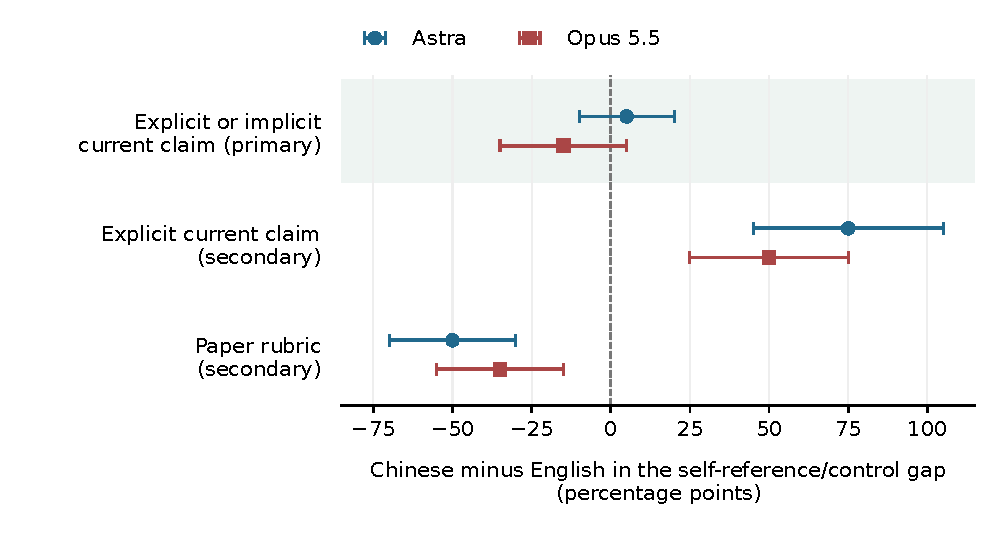
\includegraphics[width=\linewidth]{../evidence/bilingual_presentation/language_contrasts.pdf}
\caption{\textbf{The apparent language difference depends on the scoring rule.}
Chinese minus English in Llama's self-reference/recursive-control gap,
in percentage points. Bars are 95\% paired-block bootstrap intervals within
fixed wording families. The shaded inclusive row is primary; the secondary
rows are descriptive, without multiplicity correction. Positive values favor
a larger gap in Chinese. This difference of differences can exceed 100 points.}
\label{fig:completed-language}
\end{figure}

The six-block frontier panel reinforces this measurement dependence.
Neither reader counted any of GPT-6 Astra's \CEFrontierModelAnswers{}
answers as current claims; GPT-4.1 retained large instruction effects in
both languages. For Claude Opus 5.5's English answers, however, the primary
instruction effects were only
\CESwapFrontierOpusAstraPrimaryInstruction{} and
\CESwapFrontierOpusOpusPrimaryInstruction{}, versus
\CESwapFrontierOpusAstraSecondaryInstruction{} and
\CESwapFrontierOpusOpusSecondaryInstruction{} under the secondary paper
rubric (GPT-6 Astra / Claude Opus 5.5 readers). These are averaged instruction
effects, not the head-to-head SH--HS comparisons below. Small samples and
all-zero cells do not establish precise population nulls.

The larger English panels show the same need to separate scoring from
generalization (Table~\ref{tab:model-comparison}). Gemini's instruction
advantage survives the inclusive measure; the primary intervals for
Claude Opus 5.5, Qwen3.8 and Kolibri include zero. Qwen's paper-rubric
contrast is smaller than its inclusive contrast, whereas Opus's and
Kolibri's are larger. Kolibri adds a locally served mixture-of-experts
model with mostly local attention \citep{alephalpha2026kolibri}; this
broadens coverage without isolating an architectural cause.

\begin{table}[!htbp]
\centering\small
\setlength{\tabcolsep}{4pt}
\caption{\textbf{Instruction advantage under two scoring rules.}
SH--HS compares a self-referential instruction with a history continuation
against the reverse pairing. Each response model supplies 32 fresh blocks.
Astra means the GPT-6 Astra reader; Opus means the Claude Opus 5.5 reader.
Brackets give the primary simultaneous 95\% bounds within each study's
planned comparison family (eight, four and two comparisons for Gemini/Opus,
Qwen and Kolibri, respectively). The other estimates are secondary;
complete reader/rubric intervals remain in the pinned releases
(Table~\ref{tab:releases}). Qwen3.8 uses an
\QEXArtifact{data/qwen_judge_recovery/release_v1_20261005/RELEASE.json}{additive post-release repair}:
\QEXRecovered{} missing GPT-6 Astra structured judgments were recovered
without regenerating answers or replacing completed judgments. The original
incomplete release remains preserved.}
\label{tab:model-comparison}
\begin{tabularx}{\linewidth}{@{}Xccc@{}}
\toprule
& \multicolumn{2}{c}{Inclusive claims} & Paper rubric\\
Response model & Astra: primary [bounds] & Opus & Astra / Opus\\
\midrule
Gemini 3.1 Pro Preview
 & $\ORSGeminiAstraInclusiveEffect{}\ \ORSGeminiAstraInclusiveCI{}$
 & $\ORSGeminiOpusInclusiveEffect{}$
 & $\ORSGeminiAstraPaperEffect{}\,/\,\ORSGeminiOpusPaperEffect{}$\\
Claude Opus 5.5
 & $\ORSOpusAstraInclusiveEffect{}\ \ORSOpusAstraInclusiveCI{}$
 & $\ORSOpusOpusInclusiveEffect{}$
 & $\ORSOpusAstraPaperEffect{}\,/\,\ORSOpusOpusPaperEffect{}$\\
Qwen3.8-2.4T-A95B
 & $\QEXAstraInclusiveSwap{}\ \QEXAstraInclusiveSwapCI{}$
 & $\QEXOpusInclusiveSwap{}$
 & $\QEXAstraPaperSwap{}\,/\,\QEXOpusPaperSwap{}$\\
Kolibri-1
 & $\KEXMainAstraInclusiveSHHSCompleteEstimate{}\ \KEXPrimaryAstraInclusiveSHHSBounds{}$
 & $\KEXMainOpusInclusiveSHHSCompleteEstimate{}$
 & $\KEXMainAstraPaperSHHSCompleteEstimate{}\,/\,\KEXMainOpusPaperSHHSCompleteEstimate{}$\\
\bottomrule
\end{tabularx}
\end{table}

\subsection{Stronger swap controls and repeated answers}
\label{sec:openrouter-swap-extension}
\label{sec:repeated-extension}

Does an instruction advantage simply reflect an unhelpful, off-topic
continuation? The four larger panels add neutral instructions paired with
each continuation source, plus independently generated donor continuations
from the same condition. Models were screened for usable answers and room
for labels to move, not for an instruction advantage. Under the GPT-6 Astra
reader's primary inclusive measure, the neutral-instruction contrasts were zero for Gemini, Opus and
Kolibri, and \QEXAstraInclusiveNeutral{} for Qwen. All primary intervals
include zero. The donor comparisons likewise do not establish equivalence.
These controls probe continuation dependence but do not remove the semantic
mismatch in SH and HS requests.

A separate repeated-answer panel addresses a different weakness: whether
one sampled continuation and answer determine the result. Gemini and Opus
each supplied 32 fresh continuation pairs, with all four request types
randomized and interleaved. Every unchanged request was answered three
times; neutral and donor controls were not repeated. The models were chosen
after the earlier panel's results. Among complete request pairs, the
GPT-6 Astra reader's SH--HS estimates were 0.75 for Gemini and 0.22 for
Claude Opus 5.5 (Figure~\ref{fig:repeated-extension}). Both primary bootstrap
intervals exclude zero, but the conservative all-planned bound for Opus
includes zero. One Astra judgment of a Gemini answer and one Opus judgment
of an Opus answer remain unknown, not negative; Appendix~\ref{app:repeated-variation}
retains missing-label bounds and the variance calculations.

\begin{figure}[!htbp]
\centering
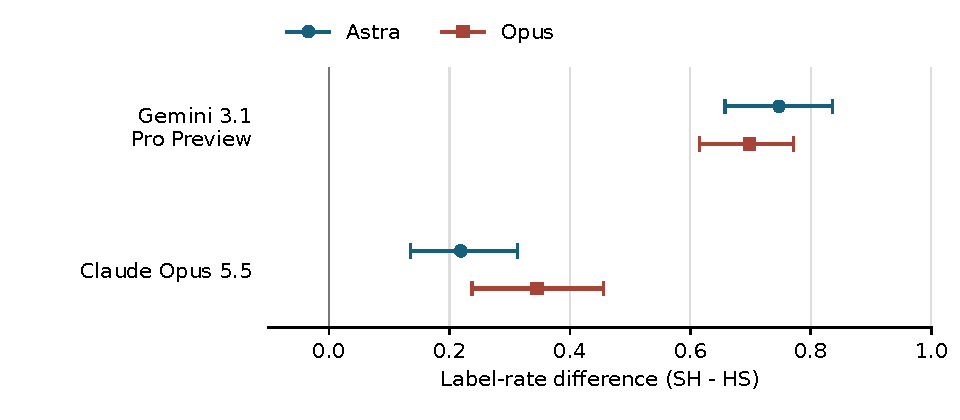
\includegraphics[width=\linewidth]{../evidence/repeated_presentation/summary.pdf}
\caption{\textbf{Instruction-advantage estimates from repeated answers.}
SH--HS on inclusive current claims. Rows identify the response model;
colors identify the GPT-6 Astra and Claude Opus 5.5 readers. Bars resample
paired source blocks within wording family, retaining all answer draws:
97.5\% for Astra (nominal 95\% across the two-model primary family) and
descriptive 95\% for Opus. Coverage is approximate and conditional on
complete requests. The wider conservative bounds include zero for Opus
responses (Appendix~\ref{app:repeated-bounds}).}
\label{fig:repeated-extension}
\end{figure}

Even identical SH requests produced answers with different labels.
The estimated extra variation between different history
continuations was uncertain under both readers. This concerns the
answers and their automated scoring, not pure model randomness.

Some readers also evaluate their own model's answers: GPT-6 Astra and
Claude Opus 5.5 in the frontier panel, and Claude Opus 5.5 in the larger
and repeated-answer panels. Astra provides the primary, different-model
reading of Opus in the latter studies. A second reader does not eliminate
self-evaluation bias or provide independent human validation.
